\documentclass[11pt]{article}
\usepackage[margin=1in]{geometry}
\usepackage{amsmath,booktabs,graphicx,hyperref}
\usepackage{xurl}
\hypersetup{hidelinks}
\graphicspath{{../figures/}{figures/}}
\title{Comparing Equal-Mass Beam Geometries}
\author{Gabriel Cirker\\\small University of Michigan, Ann Arbor\\\small \href{mailto:gcirker@umich.edu}{gcirker@umich.edu}}
\date{}
\begin{document}\maketitle
\begin{abstract}
This study compares the deflection and ideal axial buckling loads of three equal-mass beams. A solid rectangle, a hollow box and a parabolically tapered rectangle are modeled using Euler--Bernoulli beam elements. Under the dimensions chosen here, the hollow section is stiffest, while the tapered beam outperforms the baseline solid beam. These results describe an idealized comparison, not an optimized bridge design.
\end{abstract}
\section{Background and scope}
The stiffness of a beam depends on the distribution of material about the neutral axis. A hollow section can achieve a larger second moment of area when its external envelope is allowed to grow, while tapering can place material where the transverse bending moment is greatest. These design choices are constrained by loading, fabrication and local stability. Nishiyama and Sato studied nonlinear bending of tapered hollow cylindrical cantilevers, a different loading and geometry from the present linear model \cite{nishiyama}. Sepahpour and Chang compare variable-section and prismatic beams in an educational experimental context \cite{sepahpour}. These studies motivate the comparison but do not validate the present numerical predictions.

\section{Model and method}
Each steel beam has length $L=1$ m, modulus $E=200$ GPa, density $7850$ kg/m$^3$ and mass 6.28 kg. The solid baseline is 20 mm wide and 40 mm deep. The hollow section has a 40 mm by 60 mm outer envelope and a uniform wall thickness selected to match the baseline area. The tapered section has constant width and depth $h(x)=h_0[1-0.5(2x/L-1)^2]$, with $h_0$ selected to match the mass.

Pinned supports are used at both ends. A transverse load of 1000 N acts at midspan. For variable stiffness the beam equation is $(EI(x)y'')''=q$. Cubic Hermite elements discretize the bending energy, with two-point quadrature. A separate linear elastic eigenvalue analysis estimates the first axial buckling load. Deflection and axial buckling are different load cases.
\section{Geometry and equal-mass constraint}
For a rectangle of breadth $b$ and depth $h$, $A=bh$ and $I=bh^3/12$. For a box of outer dimensions $b_o,h_o$ and wall thickness $t$, the corresponding quantities are
\begin{equation}
 A=b_oh_o-(b_o-2t)(h_o-2t),\quad I=\frac{b_oh_o^3-(b_o-2t)(h_o-2t)^3}{12}.
\end{equation}
The baseline area is $8\times10^{-4}$ m$^2$. Setting the box area equal to this value gives $t=[b_o+h_o-\sqrt{(b_o+h_o)^2-4A}]/4$, approximately 4.384 mm for the stated envelope. This larger envelope is necessary: keeping the baseline envelope while removing material cannot preserve its area.

For the parabolic section, integrating its depth gives $M=\rho bLh_0(1-\alpha/3)$, and thus $h_0=h/(1-\alpha/3)$ at equal mass and width. The selected $\alpha=0.5$ gives $h_0=48$ mm and end depth 24 mm. These are prescribed designs rather than outcomes of an optimization search. An earlier manuscript compared a hollow section inside the solid baseline's original envelope and reported 0.248 mm solid deflection. Its equal-area constraint cannot be met with a nonzero cavity inside that envelope, and its fourth-derivative stencil does not reproduce the simply supported analytical deflection. The revised comparison changes the box envelope and uses the variational beam formulation below; its numerical results should therefore be read as a corrected, differently constrained comparison rather than a direct reproduction of the earlier table.

\section{Variational formulation and numerical verification}
Let $v$ be an admissible virtual transverse displacement. The static weak form is
\begin{equation}\int_0^L EI(x)y''v''\,dx=P v(L/2),\end{equation}
with zero displacement at the supports; zero end moment is the natural boundary condition. The cubic Hermite interpolation carries displacement and slope at each node. For a unit compressive axial force the geometric bilinear form is $\int_0^L y'v'\,dx$; the smallest generalized eigenvalue of bending stiffness against geometric stiffness estimates the ideal pinned-column critical load. No interaction between transverse loading and axial buckling is calculated.

The solid analytical comparison checks both support conditions and units. The tapered values at 40 and 80 elements are 0.688012 and 0.688012 mm at displayed precision, and 276.6637 and 276.6631 kN. Executable tests in \texttt{tests/} reproduce the checks. The numerical model omits geometric and material nonlinearity, local plate instability and imperfections. The mesh study measures numerical discretization sensitivity only.

\section{Results and checks}
\begin{center}\begin{tabular}{lrrr}\toprule
Section & Maximum deflection (mm) & Buckling load (kN) & Load/weight \\\midrule
Solid & 0.9766 & 210.552 & 3418 \\
Hollow & 0.2815 & 730.450 & 11857 \\
Tapered & 0.6880 & 276.663 & 4491 \\\bottomrule\end{tabular}\end{center}
The 80-element solid beam agrees with the closed-form midspan deflection $PL^3/(48EI)$ and Euler load $\pi^2EI/L^2$. For the tapered beam, refining from 40 to 80 elements changes the maximum deflection by less than 0.001\% and the buckling load by less than 0.001\%. These checks support numerical consistency, not experimental validation.
\begin{figure}[ht]\centering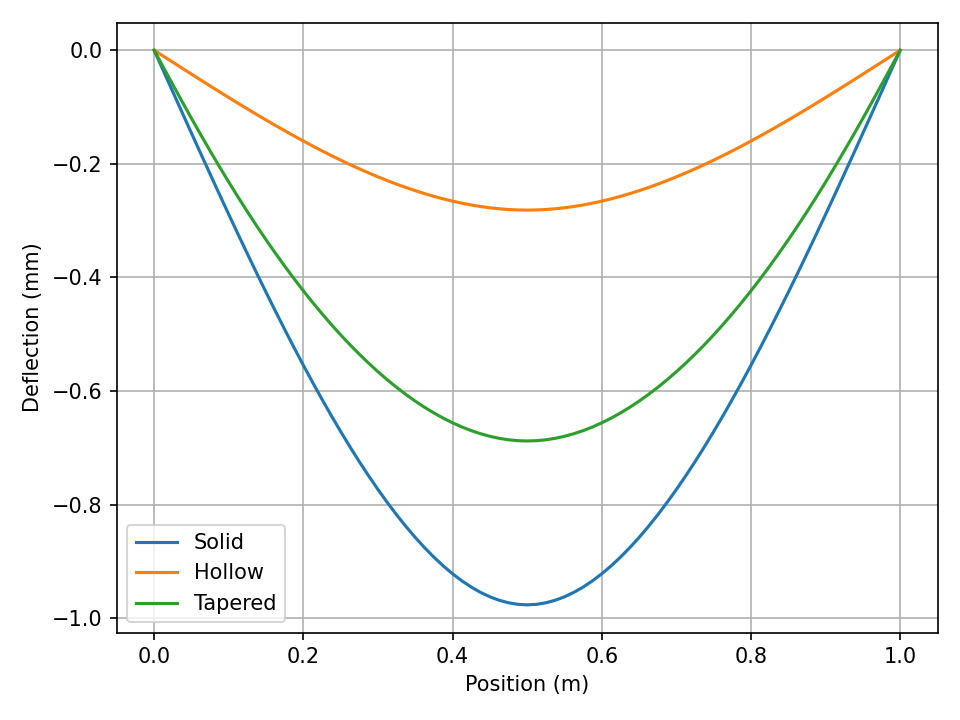
\includegraphics[width=.8\textwidth]{deflection_plot.png}\caption{Deflection under the transverse midpoint load.}\end{figure}
\section{Discussion}
The larger hollow envelope places material farther from the neutral axis and provides the greatest bending stiffness among these particular sections. Its advantage depends on the allowed outer dimensions. The tapered section places more material near midspan, where bending moment is highest. Neither result establishes a global optimum. The load-to-weight ratio uses the ideal axial buckling load and is not a general measure of structural strength. Local wall buckling, yielding, shear deformation, connections, imperfections and fabrication are outside this model. Physical tests and additional design constraints would be needed for a practical bridge comparison.

\section{Conclusion}
This comparison shows how the selected cross-sectional geometries affect stiffness and ideal elastic stability at equal mass. The hollow section benefits from its larger envelope, while the tapered section improves the baseline response under the specified cases. Further work should examine constrained geometry, local instability, yielding and experimental measurements before these results are used in design.

\begin{thebibliography}{9}
\bibitem{nishiyama} R. Nishiyama and M. Sato, ``Structural rationalities of tapered hollow cylindrical beams and their use in Japanese traditional bamboo fishing rods,'' \emph{Scientific Reports}, 12, 2448, 2022. \url{https://doi.org/10.1038/s41598-022-06426-x}.
\bibitem{sepahpour} B. Sepahpour and S. R. Chang, ``Comparison of the Strength To Weight Ratio of Variable Section Beams with Prismatic Beams,'' ASEE Annual Conference, 2007. \href{https://peer.asee.org/comparison-of-the-strength-to-weight-ratio-of-variable-section-beams-with-prismatic-beams}{ASEE proceedings}.
\end{thebibliography}

\end{document}
